\documentclass[10pt,utf8]{beamer}

\mode<presentation> {
  \usetheme{Madrid}
  \setbeamercovered{transparent}
}

\usepackage{palatino}
\usepackage{graphicx}
\usepackage{array}
\usepackage{color}
\usepackage{subfigure}
\usepackage{colortbl}
\usepackage{amsmath}
\usepackage{hyperref}
\usepackage{listings}
\usepackage{fancyvrb}

\setbeamertemplate{caption}{\raggedright\insertcaption\par} %turn off caption prefix ("Figure")

\definecolor{delim}{RGB}{20,105,176}
\definecolor{numb}{RGB}{106, 109, 32}
\definecolor{string}{rgb}{0.64,0.08,0.08}

\lstdefinestyle{java}{
	basicstyle          = \normalsize\ttfamily,
	language            = java,
	numbers             = left,
	numberstyle         = \small,
	stepnumber          = 1,
	numbersep           = 5pt,
	backgroundcolor     = \color{white},
	showspaces          = false,
	showstringspaces    = false,
	showtabs            = false,
	frame               = single,
	tabsize             = 2,
	captionpos          = b,
	breaklines          = true,
	breakatwhitespace   = false,
	morestring          = [b]",
	stringstyle         = \color{blue},
	keywordstyle        = \color{magenta},
	commentstyle        = \color{gray},
	identifierstyle     = \color{black},
	moredelim           = **[is][\bfseries]{`}{`},
	moredelim           = **[is][\color{magenta}]{$}{$}, 
	fancyvrb            = true,
}


\title{Open table format and Iceberg}
\author{Vojtěch Juránek}
\institute[Red Hat]{Red Hat}
\date{Nov 21st 2025, Debezium F2F meeting, Prague}

\newenvironment{mylisting}
{\begin{list}{}{\setlength{\leftmargin}{1em}}\item\scriptsize\bfseries}
{\end{list}}

\newenvironment{mytinylisting}
{\begin{list}{}{\setlength{\leftmargin}{1em}}\item\tiny\bfseries}
{\end{list}}


\begin{document}

\begin{frame}
    \titlepage
\end{frame}

% \begin{frame}
%     \frametitle{Terminology}
%     \begin{itemize}
%         \item \textbf{Data warehouse} - aggregates data from various sources into a central data store optimized for querying and analysis
%         \begin{itemize}
%             \item data are usually loaded using ELT/ETL (extract, transform, load) pipelines
%             \item data can be directly (without any additional pre-processing) queried and used analytics
%             \item typically provides weaker guarantees about data consistency compared to relational databases
%             \item OLAP workloads
%         \end{itemize}
%         \item \textbf{Data lake} - a centralized repository that stores vast amounts of raw data in its native format, including structured, semi-structured, and unstructured data
%         \begin{itemize}
%             \item various data types (structures, semi-structured as well as unstructured files)
%             \item uses native/original/raw data format
%             \item ability to handle huge amount of data
%         \end{itemize}
%         \item \textbf{data lakehouse} - a unified data management architecture that combines the flexibility of a data lake with the structure and features of a data warehouse
%     \end{itemize}
% \end{frame}

\begin{frame}
    \frametitle{Evolution}
    \begin{figure}
        \centering
        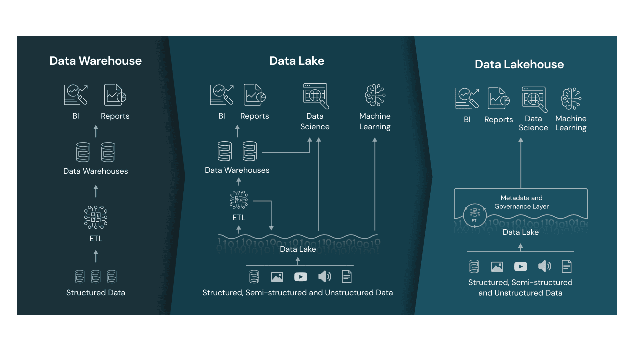
\includegraphics[height=6.5cm]{./img/data_stores.eps}
        \caption{\tiny{Source: \url{https://www.databricks.com/glossary/data-lakehouse}}}
    \end{figure}
\end{frame}

\begin{frame}
    \frametitle{Data Lakehouse}
    \begin{itemize}
        \item Supports all data types
        \item Flexible schema
        \item Cost-effective storage
        \item Real-time data processing
        \item Ideal for ML/AI workloads
    \end{itemize}
\end{frame}


\begin{frame}
    \frametitle{Open table formats}
    \begin{itemize}
        \item Standards for storing tabular data, built on top of existing file formats like Parquet, ORC or Avro.
        \item Tabular data is stored in ordinary files.
        \item Besides data itself, also metadata about the tabular data is stored in other files/directories.
        \item Open table format is basically a standard of this metadata layer.
        \item This metadata layer allows to work with a set of ordinary Parquet/ORC files like with a database table and query it.
    \end{itemize}
\end{frame}

\begin{frame}
    \frametitle{Open table formats features}
    \begin{itemize}
        \item Fast queries.
        \item ADIC transactions.
        \item Schema evolution.
        \item Support for streaming I/O (ingestion of streaming data).
        \item Time travel.
    \end{itemize}
\end{frame}

\begin{frame}
    \frametitle{Open table formats}
    Main open table formats:
    \begin{itemize}
        \color{blue} 
        \item \href{https://delta.io/}{Delta Lake}
        \item \href{https://hudi.apache.org/}{Apache Hudi}
        \item \href{https://iceberg.apache.org/}{Apache Iceberg}
        \color{black} 
    \end{itemize}
\end{frame}

\begin{frame}
    \frametitle{Open table format unification}
    Attepts to unify (not only) open table formats, e.g. \color{blue}\href{https://www.unitycatalog.io/}{Unity catalog}\color{black} (Databricks)
    \begin{figure}
        \centering
        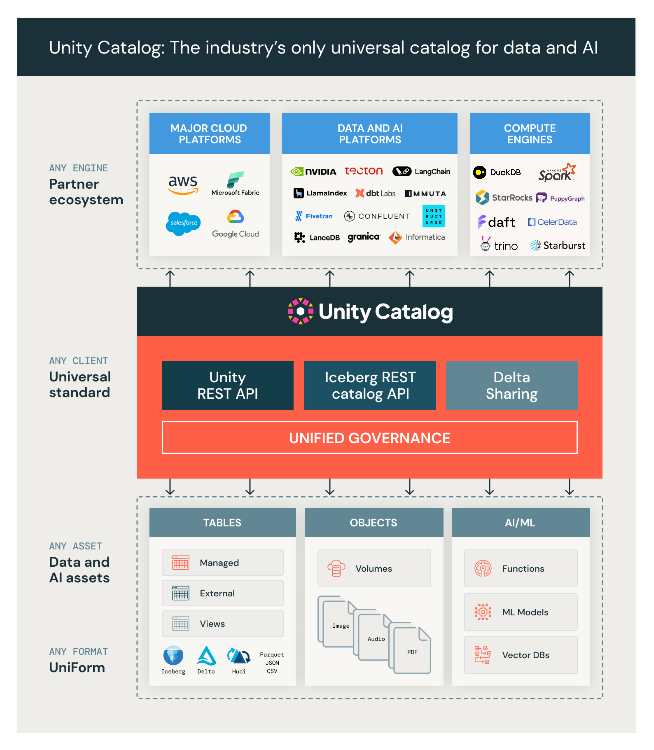
\includegraphics[height=7cm]{./img/unity.eps}
        \caption{\tiny{Source: \url{https://github.com/unitycatalog/unitycatalog}}}
    \end{figure}
\end{frame}

\begin{frame}
    \frametitle{Iceberg}
    \begin{itemize}
        \item One of the open table formats.
        \item Developed by Netflix and open-sourced in 2017.
        \item Supported by all major query/data processing engines like Spark, Trino, Flink, Hive etc. (including IBM watsonx.data).
        \item Possible winner in open table formats adoption.
    \end{itemize}
\end{frame}

\begin{frame}
    \frametitle{Iceberg}
    \begin{itemize}
        \item Metadata layer between storage and compute (query engines).
        \item Takes snapshots of data in particular point in time - created meta-meta data.
        \item Manifests describe the data in Parquet files on the blob storage.
        \item Metadata describe the data (schema, layout, location etc.) in one particular point in time.
        \item Iceberg catalog tracks metadata.
    \end{itemize}
\end{frame}

\begin{frame}
    \frametitle{High level view}
    \begin{figure}
        \centering
        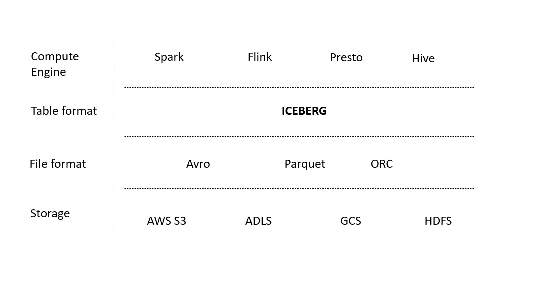
\includegraphics[height=5cm]{./img/arch.eps}
        \caption{\tiny{Source: \url{https://medium.com/geekculture/open-table-formats-delta-iceberg-hudi-732f682ec0bb}}}
    \end{figure}
\end{frame}

\begin{frame}
    \frametitle{Iceberg architecture}
    \begin{figure}
        \centering
        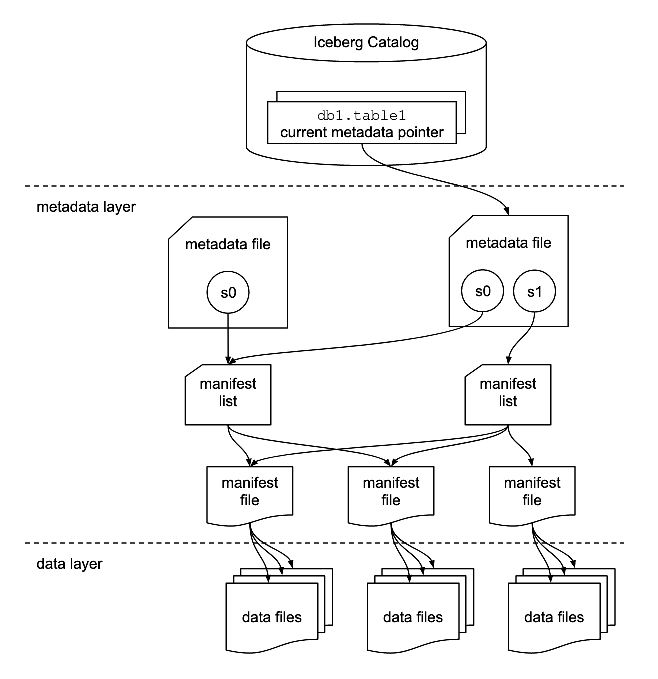
\includegraphics[height=7cm]{./img/iceberg_schema.eps}
        \caption{\tiny{Source: \url{https://iceberg.apache.org/spec/}}}
    \end{figure}
\end{frame}

\begin{frame}
    \frametitle{Catalogs}
    \begin{itemize}
        \item Catalog is top-level layer which handles queries, table creation or other DDLs. 
        \item Many implementation, written in various languages and using various backends (files, databases, REST).
        \item REST catalog specifications - allow easy implementations in various languages.
        \item Iceberg deployment can use one or many catalogs.
    \end{itemize}
\end{frame}

\begin{frame}
    \frametitle{Iceberg catalog implementation (incomplete list)}
    \begin{itemize}
     \item \color{blue}\href{https://projectnessie.org/}{Nessie}\color{black}
     \begin{itemize}
        \item Git-inspired data version control (branches, merge of branches etc).
        \item Build on top of Quarkus.
     \end{itemize}
     \item \color{blue}\href{https://polaris.apache.org/}{Apache Polaris}\color{black}
     \item \color{blue}\href{https://www.unitycatalog.io/}{Unity}\color{black}
     \item \color{blue}\href{https://docs.lakekeeper.io/}{Lakekeeper}\color{black}
     \item \color{blue}\href{https://aws.amazon.com/glue/}{AWS Glue}\color{black}
     \item  $\dots$
    \end{itemize}
    
\end{frame}

\begin{frame}
    \frametitle{Query engines integration (incomplete list)}
    \begin{itemize}
        \item Apache Spark
        \item Apache Flink
        \item Trino
        \item Apache Hive
        \item Snowflake
        \item StartRocks
        \item Google BigQuery
        \item  $\dots$
    \end{itemize}
\end{frame}

\begin{frame}
    \centering
    \huge{\textbf{Demo - Iceberg 101}}
\end{frame}

\begin{frame}
    \frametitle{Debezium server Iceberg sink}
    \begin{figure}
        \centering
        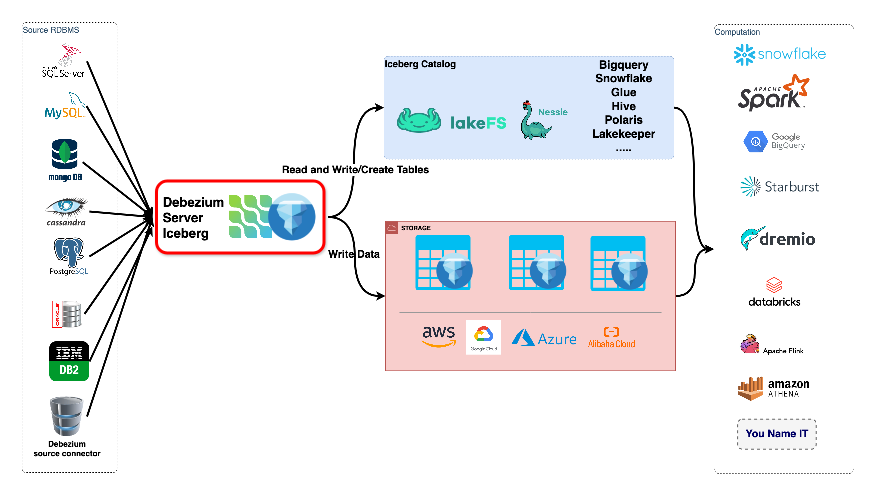
\includegraphics[height=6.5cm]{./img/dbz_icebeg.eps}
        \caption{\tiny{Source: \url{https://github.com/memiiso/debezium-server-iceberg}}}
    \end{figure}
\end{frame}

\begin{frame}
    \centering
    \huge{\textbf{Demo - Debezium server Iceberg sink}}
\end{frame}

\begin{frame}
    \frametitle{Questions?}
    \centering
     \textbf{\Huge{Thank you!}}
    
    \vspace{1.5cm}
    
    \textbf{\Huge{Questions?}}
    
    \vspace{1cm}
\end{frame}

%%%%%%%%%%%%%%%%%%%%%%%%%%%%%%%%%%%%%%%%%%%%%%%%%%%%%%%%%%%%%%%%%%%%%%%%%%%%%%%%%%%%%%%%%%%%%%%%%
%%% BACKUP
%%%%%%%%%%%%%%%%%%%%%%%%%%%%%%%%%%%%%%%%%%%%%%%%%%%%%%%%%%%%%%%%%%%%%%%%%%%%%%%%%%%%%%%%%%%%%%%%%

% \begin{frame}
%     \centering
%     \huge{\textbf{Backup slides}}
% \end{frame}

\end{document}
